%\documentclass[compress, draft]{beamer}
\documentclass[compress]{beamer}
\mode<presentation>
{}
\usepackage{amsmath, amssymb, amsbsy, mathrsfs, empheq}
\usepackage{xmpmulti}
\usepackage[latin1]{inputenc}
\usepackage{graphicx}
\usepackage{bbding}
\usepackage[controls]{animate}
%\usepackage{beamerthemesplit}
\usepackage[style=authoryear-comp, backend=bibtex]{biblatex}
\renewbibmacro{in:}{}
\bibliography{mybib}

%\useoutertheme[subsection=false]{smoothbars}
%\usetheme{Amsterdam}
\setbeamertemplate{navigation symbols}{}
\setbeamertemplate{footline}[frame number]

\newcommand{\vs}[1]{\boldsymbol{#1}}   
\newcommand{\abs}[1]{\left| #1 \right|}

\mode<presentation>
\title{Oscillatory deformation of amorphous materials: \\ a numerical investigation}
\author{Davide Fiocco}
%\date{PhD private defense \\ \vspace{0.5cm} EPFL, January 17, 2014}
\date{PhD private defense \\ \vspace{0.5cm} EPFL, \today}

\begin{document}
	
	\begin{frame}[t, plain, noframenumbering]
		\titlepage
	\end{frame}
	
	\begin{frame}{My thesis in a nutshell}
	
		 Study the behavior of model \textbf{metallic glasses} under deformation, by means of atomistic computer simulations
	
		\begin{figure}
			\animategraphics[width=0.4\textwidth, buttonsize = 0.35cm, loop]{12}{Graphics/ShearedGlassPOV/cube}{01}{31}
			\caption{Shear strain $\gamma = \tan \theta$ is varied between $-\gamma_{max}, \gamma_{max}$}
		\end{figure}
	
		\begin{enumerate}
			\item<2-> What happens in the deformed glass at a microscopic level? \\
			\item<3-> Are there any similarities with other systems?\\
		\end{enumerate}
		
	\end{frame}
	
	\section{Introduction to metallic glasses}
	
	\begin{frame}{What is a metallic glass?}
		
		\begin{block}{Manufacturing of a metallic glass}
			
			\begin{enumerate}
				\item<1-> Take a melt of transition metals (e.g. Zr, Al, Ni and Cu)
				\item<2-> Quench it fast enough so to avoid crystallization  
				\item<3-> A glass transition can happen: the result is a solid with no long range order
			\end{enumerate}
			
			\onslide<4->
			
			If bulk samples are obtained one has a bulk metallic glass
			
		\end{block}
		
		\onslide<5->
		
		\begin{block}{Mechanical properties of metallic glasses for applications}
			
			\begin{itemize}
				\item<6-> Elastic behavior up to large values of strain\hspace{0.2cm} {\color{green} \Checkmark}
				\item<7-> Low losses\hspace{0.2cm} {\color{green} \Checkmark}
				\item<8-> Corrosion resistance\hspace{0.2cm} {\color{green} \Checkmark}
				\item<9-> Brittle failure\hspace{0.2cm} {\color{red} \XSolidBrush}
			\end{itemize}
	
		\end{block}
		
	\end{frame}
	
	\subsection{Modelization of metallic glasses}
	
	\begin{frame}{How can one model a metallic glass?}
		
		\onslide<2->
		
		\begin{block}{The role of microscopic (atomistic) descriptions}
			
			Input and benchmarks for mesoscopic descriptions (e.g. STZ)
		
		\end{block}
		
		\onslide<3->
		
		\begin{block}{Examples of microscopic models}
			
			\begin{itemize}
				\item Embedded Atom Potentials (EAM)
				\item Lennard-Jones mixtures (LJ)
			\end{itemize}
			
		\end{block}
		
		\onslide<4-> One can then unleash the arsenal of numerical integration methods
		
	\end{frame}

	\begin{frame}{Simulating glasses with LJ binary mixtures}
		
		\onslide<2->
		
		\begin{block}{Tuning of the LJ interaction potential}
	
			Parameters in the potential
			
			\begin{equation*}
				\phi_{ij}(r) = 4\epsilon_{ij} \left(\left(\frac{\sigma_{ij}}{r}\right)^{12} - \left(\frac{\sigma_{ij}}{r}\right)^{6}\right)
			\end{equation*}
	
			are chosen so to make the system less prone to crystallization/phase separation
	
		\end{block}
		
		\onslide<3->
		
		\begin{block}{Making of the glass: quenching at infinite rate}
	
			\onslide<4->
	
			\begin{columns}[c]
				
				\begin{column}{0.25\textwidth}
					\centering
					\begin{figure}
						\multiinclude[<+>][format=png, start = 0, end = 6, graphics={width=\columnwidth}]{Graphics/Quench/quench}
					\end{figure}
				\end{column}
			
				\begin{column}{0.75\textwidth}
				
					\begin{enumerate} 
						\item<4-> The system can be equilibrated at constant $T$ with a Nos\'e-Hoover thermostat
						\item<5-> Velocities are disregarded \\ \onslide<6->  and configurations are energy minimized with a conjugate-gradient algorithm
					\end{enumerate}
				
				\end{column}
				
			\end{columns}
	
		\end{block}		
		
	\end{frame}	

	\begin{frame}{Properties of undeformed samples}

		\begin{block}{}

			Energy minimization of configurations equilibrated at $T$ yields \emph{inherent structures} with \emph{effective temperature} $T$

			\begin{columns}[T]
				
				\begin{column}{0.3\textwidth}
					\centering{}
					\vspace{0.5cm}
					\begin{figure}
						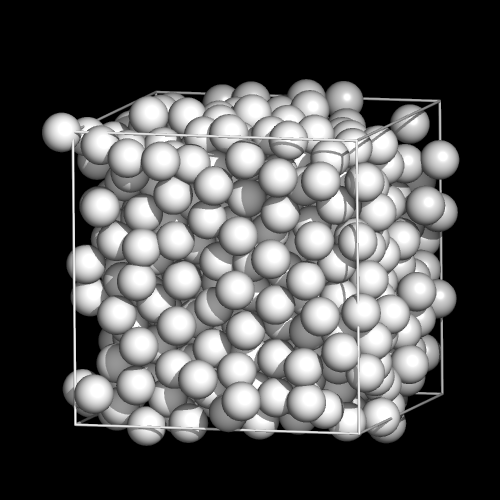
\includegraphics[width=0.9\columnwidth]{Graphics/Quench/quench-5}
					\end{figure}
				\end{column}

				\onslide<2->

				\begin{column}{0.7\textwidth}
					\begin{figure}
						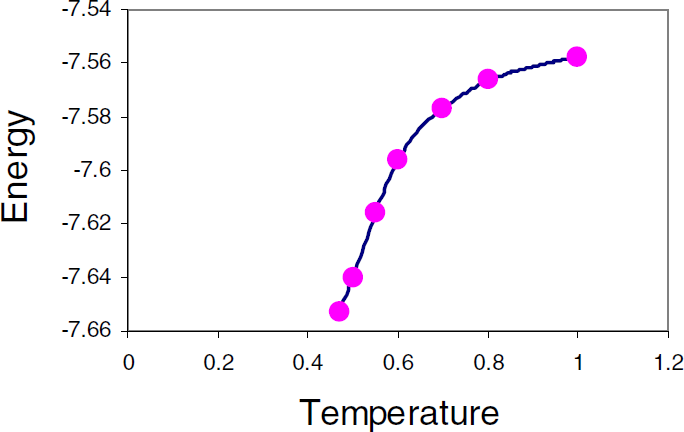
\includegraphics[width=0.8\columnwidth]{Graphics/Literature/EnergyvsT}
						%\caption{Data taken from Lacks and Osborne, 2004}
					\end{figure}
				\end{column}
			
			\end{columns}
			
		\end{block}
		
		\vspace{0.5cm}
		
		The properties of the inherent structures depend on the effective $T$
		
		\vspace{0.3cm}
		
		\onslide<3-> How to deform them?
		
	\end{frame}

	\section{Simulations of deformation of metallic glasses}
	
	\subsection{Oscillatory quasi static deformation protocol}

	\begin{frame}{Deformation}
		
		\begin{block}{Deformation protocol: athermal quasi-static (AQS)}
		
			\begin{columns}[T]
				
				\begin{column}{0.3\textwidth}
					\begin{figure}
						\centering
						\multiinclude[<+>][format=png, start = 2, end = 5, graphics={width=0.9\textwidth}]{Graphics/AQS/confs/aqs}
					\end{figure}
				\end{column}
			
				\begin{column}{0.7\textwidth}
				
					\vspace{0.5cm}
					
					\begin{enumerate}
						\item<2-> Affine transformation + \\ update of the boundary conditions \\ to increment the strain of $d\gamma$
						\item<3-> Energy minimization
					\end{enumerate}
				\end{column}
				
			\end{columns}
			
			\vspace{0.5cm}
			
			\begin{itemize}
				\item<4-> By iterating the steps, one can reach arbitrary strains
			\end{itemize}
			
		\end{block}
		
	\end{frame}

	\begin{frame}{What is the effect of changing the strain?}
		
		\begin{columns}[t]
			\begin{column}{0.5\textwidth}
				\begin{block}{\centering in 3D space}
					\begin{figure}
						\animategraphics[width=0.65\textwidth, buttonsize = 0.35cm]{12}{Graphics/States/Diffusing/confs/aqs}{0}{9}
					\end{figure}
				\end{block}
			\end{column}
			\begin{column}{0.5\textwidth}
				\begin{block}{\centering in ($3N$D) configuration space}
					\begin{figure}
						\animategraphics[width=0.65\textwidth, buttonsize = 0.35cm]{12}{Graphics/AQSLandscape/aqs-}{00}{15}
					\end{figure}
				\end{block}
			\end{column}
		\end{columns}

	\end{frame}

	\subsection{Known and new results}

	\begin{frame}<1>[label=Triangle]{Oscillatory strain}
		
		Consider a triangle wave strain profile ranging in $[-\gamma_{max}, \gamma_{max}]$, and define $\gamma_{acc} = \sum{\abs{d\gamma}}$

		\begin{figure}
			\multiinclude[<+>][format=pdf, start = 0, end = 9, graphics={width=\textwidth}]{Graphics/Triangle/Triangle}
		\end{figure}
		
		\onslide<3->
		
		\begin{alertblock}{What happens if the system is subjected to \emph{more} oscillations?}
			\onslide<4-> We analyse:
			\begin{itemize}
				\item<4-> \alert<7>{Potential energy per particle within the sample}
				\item<5-> \alert<8>{Particle motion}
				\item<6-> \alert<9>{Energy dissipation}
			\end{itemize}
		\end{alertblock}
		
	\end{frame}

	\begin{frame}{What is the effect of a single semicycle? }
		
		\begin{block}{Straining the sample back and forth once\footfullcite{lacks2004energy}}

			\begin{figure}
				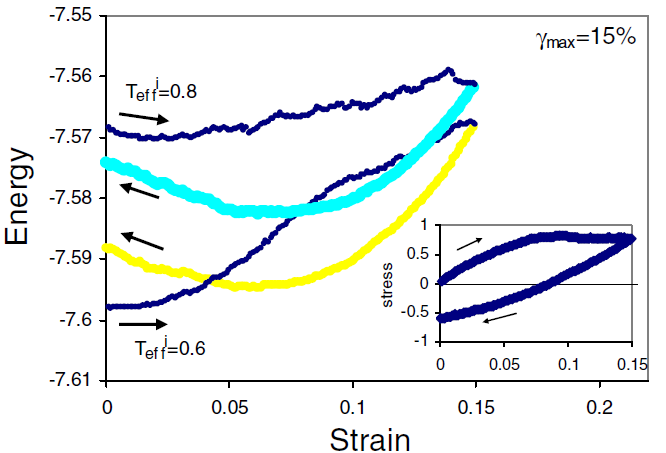
\includegraphics[width=0.5\textwidth]{Graphics/Literature/Rejuvenaging}
			\end{figure}
			
			\vspace{-0.2cm}
			
			\begin{itemize}
					\item<2-> Samples differing in their effective $T$ change their energy
					\item<3-> The result (increase or decrease) depends on $T$ (and $\gamma_{max}$)  
			\end{itemize}
			
		\end{block}
		
	\end{frame}

	\againframe<2-7>{Triangle}

	\begin{frame}{Potential energy}

		\begin{figure}
			\multiinclude[<+>][format=pdf, start = 0, end = 5, graphics={width=0.85\textwidth}]{Graphics/Graphs/EKA4000}
		\end{figure}
		
		\begin{itemize}
			\item<1-> Different regimes:
				\begin{itemize}
					\item<1-> Low $\gamma_{max}$: fixed values of $U_{\infty}$, dependence from $T$
					\item<2-> High $\gamma_{max}$: fluctuating values of $U_{\infty}$, no dependence from $T$
				\end{itemize}
			\item<4-> Energy profiles are described by stretched exponentials $$U = ( U_{0} - U_{\infty}) e^{-(\gamma_{acc}/\widetilde \gamma_{acc})^\alpha} + U_{\infty}$$
		\end{itemize}
		
	\end{frame}	

	\begin{frame}{Values of $\widetilde \gamma_{acc}$ from the energy fits}
	
		$\widetilde \gamma_{acc}$ marks the onset of a ``steady state''

		\begin{figure}
			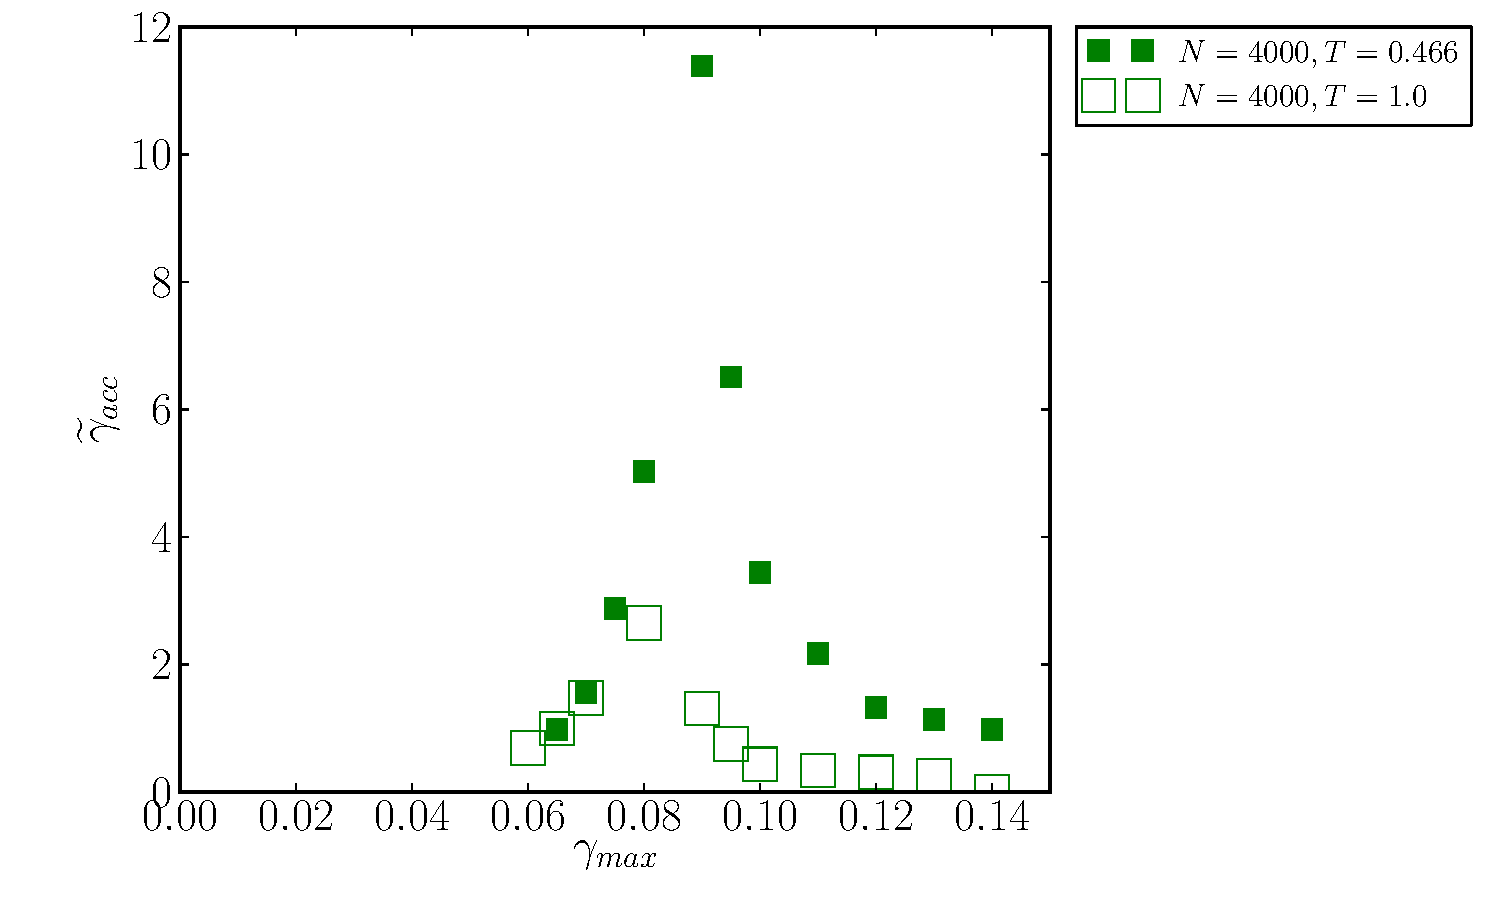
\includegraphics[width=0.85\textwidth]{Graphics/Graphs/Epeaks}
		\end{figure}
		
		\begin{itemize}
			\item $\widetilde \gamma_{acc}$ peaks for some intermediate value
		\end{itemize}
		
	\end{frame}

	\againframe<8>{Triangle}

	\begin{frame}{MSD in the asymptotic state}

		The MSD measured from samples encountered for $\gamma_{acc} > \widetilde \gamma_{acc}$

		\begin{figure}
			\multiinclude[<+>][format=pdf, start = 0, end = 2, graphics={width=0.85\textwidth}]{Graphics/Graphs/MSDRelaxKA4000}
		\end{figure}
		
		\begin{itemize}
			\item<1-> Two regimes:
				\begin{itemize}
					\item<1-> Low $\gamma_{max}$: samples do not move at all (absorbing)
					\item<2-> High $\gamma_{max}$: samples diffuse
				\end{itemize}
			\item<3-> The trends can be fit with: MSD = $D (\gamma_{acc} - \widetilde \gamma_{acc})$ 
		\end{itemize}
		
	\end{frame}

	\begin{frame}{Values of $D$ extracted from the MSD}

		\begin{figure}
			\multiinclude[<+>][format=pdf, start = 0, end = 2, graphics={width=0.85\textwidth}]{Graphics/Graphs/D}
		\end{figure}
		
		\begin{itemize}
			\item<1-> A transition at a value $\gamma_{c}$
			\item<2-> $D \propto (\gamma_{max} -\gamma_{c})^{\beta}$?
		\end{itemize}
		
	\end{frame}

	\begin{frame}{Scaling of $\gamma_{c}$}

		\begin{figure}
			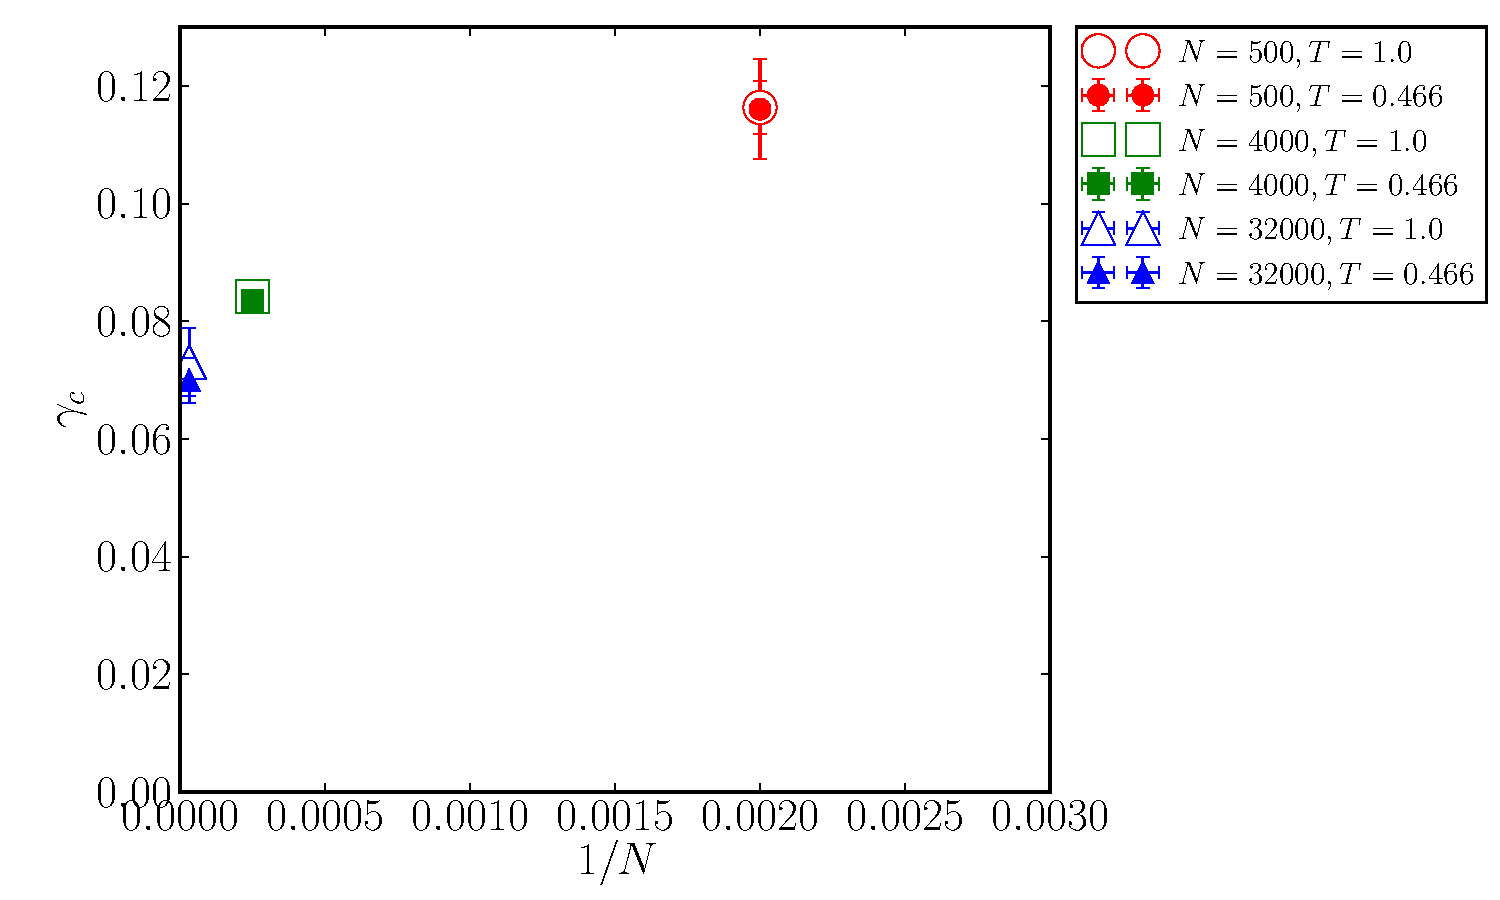
\includegraphics[width=0.85\textwidth]{Graphics/Graphs/GammacScaling}
		\end{figure}
		
		The putative $\gamma_{c}$ seems not to be vanishing for $N \to \infty$
		
	\end{frame}

	\againframe<9>{Triangle}
	
	\begin{frame}{Hysteresis curves in the ``steady state''}

		\begin{figure}
			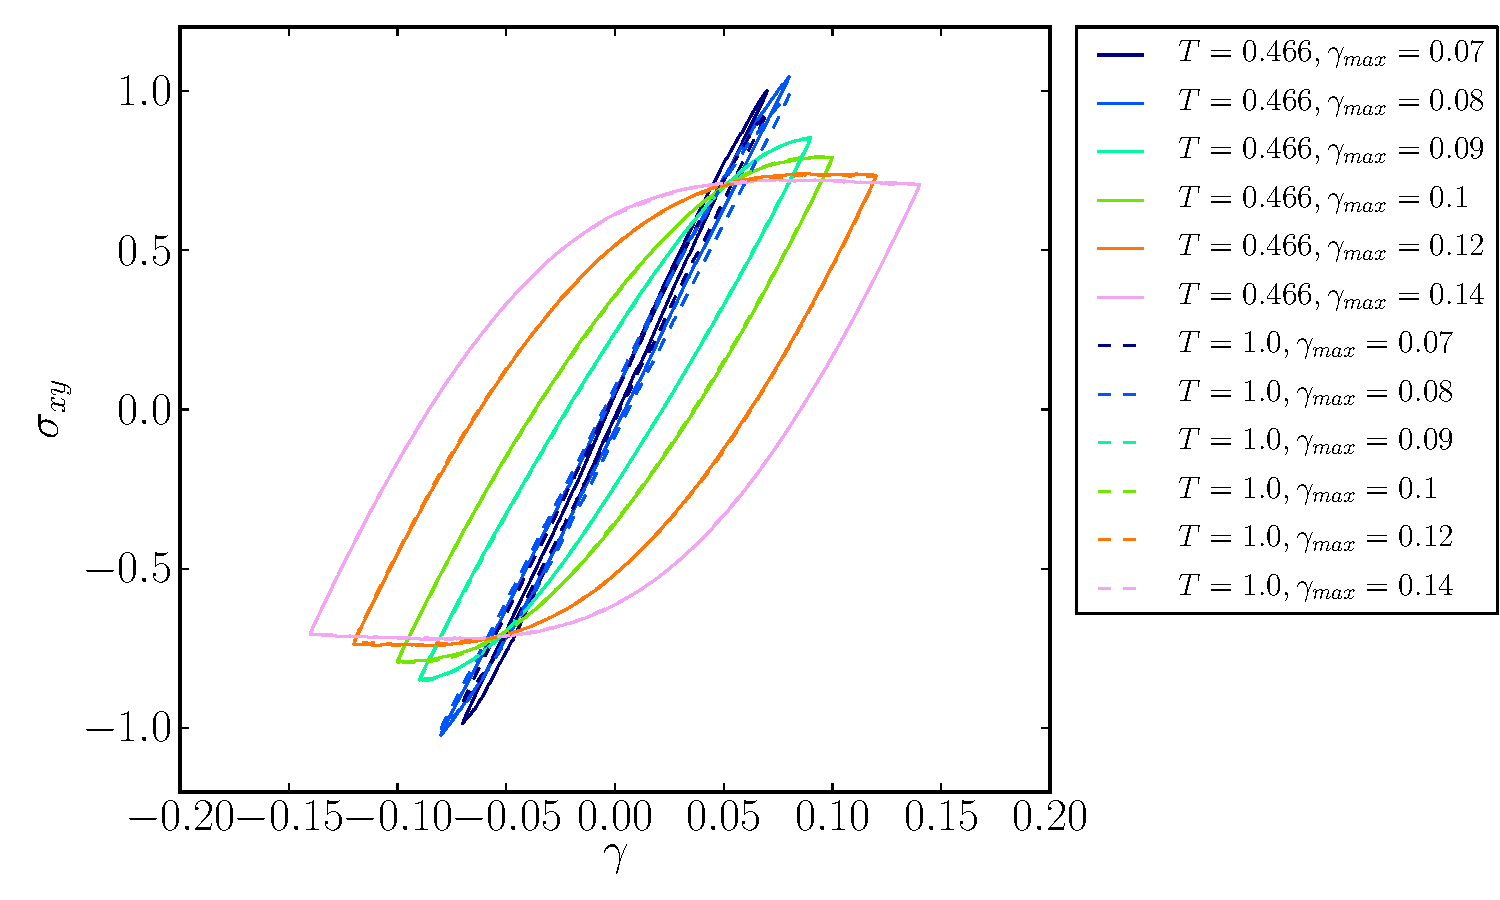
\includegraphics[width=0.85\textwidth]{Graphics/Graphs/HisteresisKA4000}
		\end{figure}

		\begin{itemize}
			\item<2-> Two regimes:
				\begin{itemize}
					\item Low $\gamma_{max}$: narrow curves
					\item High $\gamma_{max}$: broad curves
				\end{itemize}
		\end{itemize}
		
	\end{frame}

	\begin{frame}{Area of the hysteresis curves}

		\begin{figure}
			\multiinclude[<+>][format=pdf, start = 0, end = 2, graphics={width=0.85\textwidth}]{Graphics/Graphs/Dissipation}
		\end{figure}
		
		The onset of dissipation is compatible with $\gamma_{c}$ 
		
	\end{frame}

	\begin{frame}{A comparison: suspensions and their behavior\footfullcite{corte2008random}}

		\begin{figure}
		\centering
			\animategraphics[width=0.4\textwidth, buttonsize = 0.35cm, loop]{12}{Graphics/ShearedSuspensionPOV/suspension}{00}{29}
		\end{figure}

		\begin{itemize}
			\item<1-> Particles suspended in a viscous medium
			\item<2-> \emph{Active} particles collide with others during a cycle and don't come back to the initial position
			\item<3-> After some cycles the number of active particles doesn't change anymore
		\end{itemize}
	
	\end{frame}
	
	\begin{frame}{Suspensions and their behavior\footfullcite{corte2008random}: a comparison}
	
		\begin{figure}
			\onslide<1->
			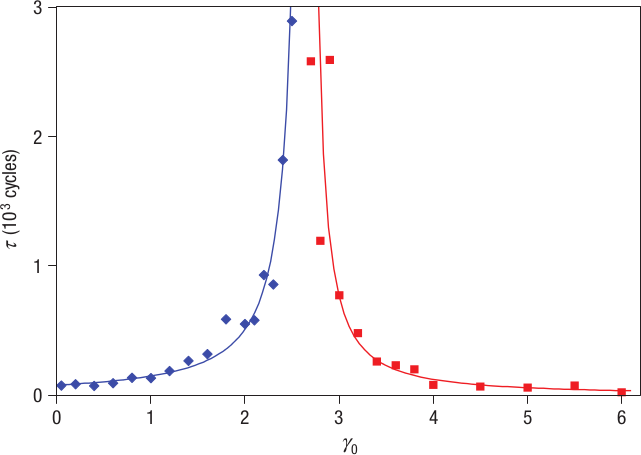
\includegraphics[scale = 0.22]{Graphics/Literature/Relaxation}	
			\hspace{1cm}
			\onslide<2->
			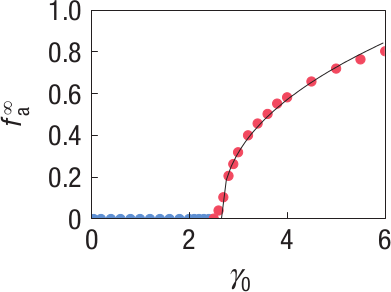
\includegraphics[scale = 0.25]{Graphics/Literature/Active}	
		\end{figure}
		
		\onslide<1->
		
		\begin{itemize}
			\item<1-> The number of cycles needed to reach the steady fraction of active particles resembles $\widetilde \gamma_{acc}$  in LJ
			\item<2-> The asymptotic fraction of active particles as a function of $\gamma_{max}$ resembles $D$ in LJ
		\end{itemize}
		
	\end{frame}
	
	\begin{frame}{Partial summary: existence of a transition}
		
		\begin{itemize}
			\item<1-> Past observations of energy changes in deformed LJ are rationalized: they are the initial steps towards an asymptotic state
			\item<2-> Evidence of a transition at $\gamma_{c}$:
				\begin{itemize}
					\item<3-> $\gamma_{max} < \gamma_{c} \rightarrow$ no diffusion, low dissipation
					\item<4-> $\gamma_{max} > \gamma_{c} \rightarrow$ diffusion, high dissipation
				\end{itemize}
			\item<5-> The scenario is qualitatively similar to that of suspensions
		\end{itemize}
		
	\end{frame}

	\subsection{Comparision with suspensions, memory phenomena}

	\begin{frame}{Pushing the analogy further: memory phenomena\footfullcite{keim2011generic}}

		\begin{columns}[T]
			\begin{column}{0.3\textwidth}
				\begin{block}{Training at $\gamma_{1}$}
					\begin{figure}
						\animategraphics[scale=0.18, buttonsize = 0.3cm, loop]{12}{Graphics/ShearedSuspensionPOV/suspension}{00}{28}
					\end{figure}
				\end{block}
			\end{column}
			\begin{column}{0.65\textwidth}
				\begin{block}{Reading at different $\gamma_{r}$}
					\begin{figure}
						\animategraphics[scale=0.18, buttonsize = 0.3cm]{12}{Graphics/ShearedSuspensionPOV/Reading1/suspension}{00}{14} 
						\animategraphics[scale=0.18, buttonsize = 0.3cm]{12}{Graphics/ShearedSuspensionPOV/Reading2/suspension}{00}{44}
					\end{figure}
				\end{block}
			\end{column}
		\end{columns}
		
		\begin{block}{Encoding and reading of memory}
			
			\begin{itemize}
				\item<2-> Samples are \emph{trained} by $N_{cyc}$ cycles of amplitude $\gamma_{1}$
				\item<3-> Trained samples are \emph{read} with one cycle of amplitude $\gamma_{r}$: the number of active particles is measured as a function of $\gamma_{r}$
			\end{itemize}
			
		\end{block}
		
	\end{frame}

	\begin{frame}{Memory phenomena in suspensions (continued)}

		\begin{columns}[c]
			
			\begin{column}{0.3\textwidth}
				\centering
				\begin{figure}
					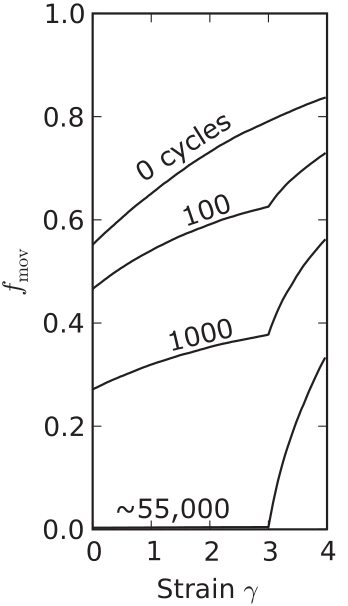
\includegraphics[height=0.6\textheight]{Graphics/Literature/SuspensionSingleMemory}
				\end{figure}
			\end{column}

			\begin{column}{0.7\textwidth}
				
				\begin{itemize}
					\item<1-> Trainings produce samples which bear a trace of $\gamma_{1}$ when read
					\item<2-> The longest trainings produce samples that don't have any active particles for cycles with $\gamma_{r} < \gamma_{1}$
				\end{itemize}

			\end{column}

		\end{columns}

		\vspace{0.5cm}
		\onslide<3->
		What happens if one applies the same protocol to a LJ sample?
				
	\end{frame}

	\begin{frame}{Single memory in LJ samples}

		Take the MSD of particles of trained samples read with $\gamma_{r}$:

		\begin{figure}
			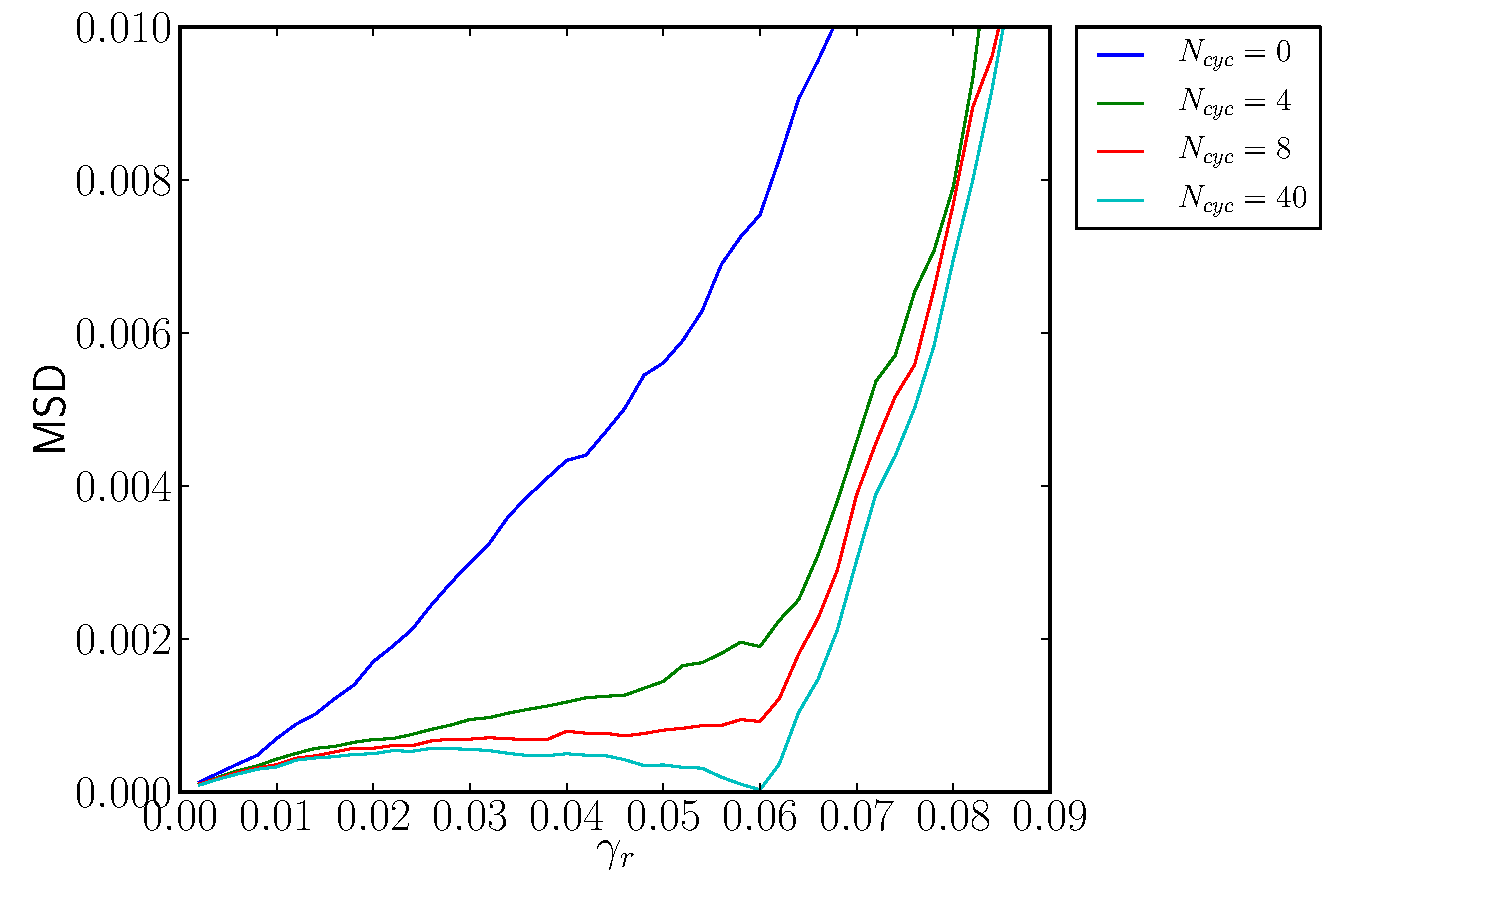
\includegraphics[width=0.85\textwidth]{Graphics/Graphs/MemoryKASingle}
		\end{figure}
		
		\begin{itemize}
			\item<2-> The behavior agrees qualitatively with that of suspensions
			\item<3-> The ``bump'': MSD $\neq 0$ if $\gamma_{r} < \gamma_{1}$, even for long trainings
		\end{itemize}
		
	\end{frame}	

	\begin{frame}{Why the bump?}
		
		\begin{columns}[t]

			\begin{column}{0.3\textwidth}
				\begin{block}{\centering $\gamma_{r} < \gamma_{1}$}
					\begin{figure}
						\animategraphics[width=\textwidth, buttonsize = 0.35cm]{8}{Graphics/States/Under/confs/aqs}{0}{24}
					\end{figure}
				\end{block}
			\end{column}

			\begin{column}{0.3\textwidth}
				\begin{block}{\centering $\gamma_{r} = \gamma_{1}$}
					\begin{figure}
						\animategraphics[width=\textwidth, buttonsize = 0.35cm]{8}{Graphics/States/Absorbing/confs/aqs}{0}{40}
					\end{figure}
				\end{block}
			\end{column}

			\begin{column}{0.3\textwidth}
				\begin{block}{\centering $\gamma_{r} > \gamma_{1}$}
					\begin{figure}
						\animategraphics[width=\textwidth, buttonsize = 0.35cm]{8}{Graphics/States/Above/confs/aqs}{0}{40}
					\end{figure}
				\end{block}
			\end{column}
			
		\end{columns}

		\begin{itemize}
			\item<1-> A sample trained at $\gamma_{1}$ returns into the original state after a reading cycle $\gamma_{r} = \gamma_{1}$, via a sequence of rearrangements
			\item<2-> If the amplitude $\gamma_{r} \neq \gamma_{1}$, the sequence is altered!
		\end{itemize}
		
	\end{frame}

	\begin{frame}{Partial summary: memory phenomena}
		
		\begin{itemize}
			\item Memory can be encoded and read in LJ samples \\ by means of oscillatory deformation
			\item There are qualitative differences with memory of suspensions
		\end{itemize}
		
	\end{frame}

	\section{Toy models}

	\begin{frame}{Can our results be generalized?}
		
		All the behavior above depends on the dynamics of the LJ system
		\begin{columns}[t]
			\begin{column}{0.5\textwidth}
				\begin{block}{\centering in 3D space}
					\begin{figure}
						\animategraphics[width=0.65\textwidth, buttonsize = 0.35cm]{12}{Graphics/States/Diffusing/confs/aqs}{0}{20}
					\end{figure}
				\end{block}
			\end{column}
			\begin{column}{0.5\textwidth}
				\begin{block}{\centering in ($3N$D) configuration space}
					\begin{figure}
						\animategraphics[width=0.65\textwidth, buttonsize = 0.35cm]{12}{Graphics/AQSLandscape/aqs-}{00}{40}
					\end{figure}
				\end{block}
			\end{column}
		\end{columns}

		\onslide<2->
		Is such behavior found in other systems with a deformable energy landscape?
		
	\end{frame}

	\begin{frame}{NK model}

		\begin{block}{A discrete energy landscape depending on a parameter $\gamma$}
		
			\footnotesize
			
			\begin{columns}[c]
				\begin{column}{0.35\textwidth}
					\centering
					\begin{figure}
						\multiinclude[<+>][format=png, start = 1, end = 12, graphics={width=\textwidth}]{Graphics/Hypercube/hypercube}
						%\animategraphics[width=\textwidth, buttonsize = 0.35cm]{6}{Graphics/Hypercube/hypercube-}{1}{23}
					\end{figure}
				\end{column}
				\begin{column}{0.65\textwidth}
					\begin{itemize}
						\item<1-> A set of connected nodes
						\item<2-> An energy function is defined for each node
						\item<3-> Inherent structures are well defined by a steepest descent algorithm
						\item<4-> The energy function depends on $\gamma$ 
						\item<8-> Steepest descent allows to perform ``athermal deformation'' as $\gamma$ is varied
					\end{itemize}
				\end{column}
			\end{columns}
		\end{block}
		\onslide<12->
		\begin{block}{Information from the NK model}
			The energy behavior, diffusion and memory effects can be studied as $\gamma$ is varied in an oscillatory way
		\end{block}
		
	\end{frame}

	\begin{frame}{Example: single memory in NK samples}

		Take the Hamming distance of trained samples read with amplitude $\gamma_{r}$:

		\begin{figure}
			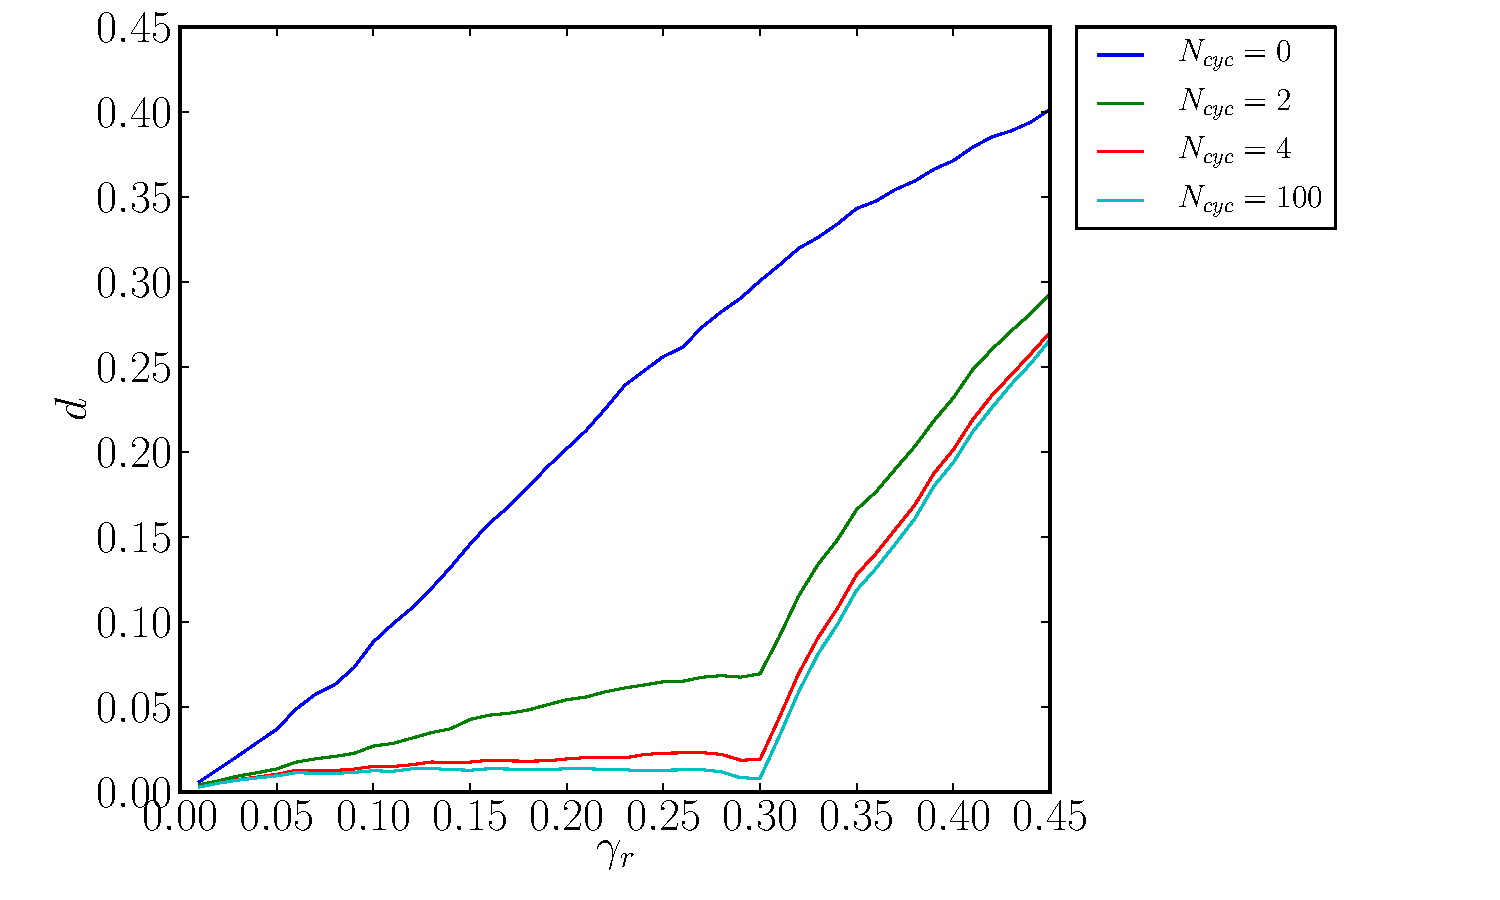
\includegraphics[width=0.85\textwidth]{Graphics/Graphs/MemoryNKSingle}
		\end{figure}
		
		\begin{itemize}
			\item The behavior agrees qualitatively with that of LJ
		\end{itemize}
		
	\end{frame}	

	%\begin{frame}{Summary of results on toy models}
	%
		%\begin{itemize}
			%\item Both the TM and the NK models are able to show 
				%\begin{itemize}
					%\item a hint of a transition at some $\gamma_{c}$ as a function of $\gamma_{max}$
					%\item memory effects
				%\end{itemize}
			%\item The results on the NK model suggest that the transition at $\gamma_{c}$ and memory effects could be observed in a wider class of systems having a deformable energy landscape
			%\item The systems examined are expected to be affected by size effects
		%\end{itemize}
	%
	%\end{frame}
%
	\begin{frame}{Conclusions}
		
		\footnotesize
		
		\begin{block}{Key results of the thesis}
			\begin{itemize}
				\item<1-> Previous observation of energy changes on oscillatory deformed LJ glasses are rationalized
				\item<2-> Deformed LJ samples show a transition similar to that seen in suspensions
				\item<3-> Deformed LJ samples display memory phenomena, with important differences w.r.t. suspensions
				\item<4-> Toy models mimic the behavior observed in LJ systems, and suggest that the phenomenology above could be observed in a wider class of systems
			\end{itemize}
		\end{block}
		
		\onslide<5->
		
		\begin{block}{Open issues}
			\begin{itemize}
				\item<6-> Quantitative characterization of the transition at $\gamma_{c}$, assessment of size effects
				\item<7-> Comparison with mesoscopic theories of deformation
				\item<8-> Link with other physical systems
			\end{itemize}
		\end{block}
		
	\end{frame}

	\begin{frame}[noframenumbering]
	
		\centering
		{\Large Thank you!}
		
		\vspace{2cm}
		
		\onslide<2->
		and to \\ G. Foffi, and S. Sastry (TIFR Hyderabad)
		
	\end{frame}

\end{document}
